\documentclass[a4paper, portuguese]{report}

\usepackage[ruled]{algorithm2e}
\usepackage{cite}
\usepackage{comment}
\usepackage{graphicx}
\usepackage{parskip}
\usepackage{minted}
\usepackage{titlesec}
\usepackage[portuguese]{babel}
\usepackage[hyphens]{url}
\usepackage[hidelinks,pdfusetitle]{hyperref}
\usepackage{xcolor}
\usepackage{siunitx}
\usepackage[utf8]{inputenc}
\usepackage[T1]{fontenc}

\hypersetup{
    breaklinks=true,
    pdfauthor={Diogo Medeiros e João Santos},
    pdftitle={Simulação de Incêndios Florestais Baseada em Agentes}
}
\urlstyle{same}

\providecommand{\keywords}[1]
{
    \small
    \textbf{\textit{Palavras-chave --}} #1
}
% define algorithm2e comments
\SetKwComment{Comment}{/* }{ */}

\setlength{\parindent}{2em}
\setlength{\parskip}{\baselineskip}
\titleformat{\chapter}[display]
{\normalfont\huge\bfseries}{\chaptertitlename\ \thechapter}{10pt}{\Huge}
\titlespacing*{\chapter}{0pt}{0pt}{30pt}

\title{\textbf{Computação Natural}\\ Mestrado em Engenharia Informática - 1.º ano\\ \vspace*{1cm} José Paulo Barroso de Moura Oliveira\\ Eduardo José Solteiro Pires\\ \vspace*{3cm}\textbf{Trabalho Prático}\\ Simulação de Incêndios Florestais Baseada em Agentes \vspace*{1cm}}
\author{Diogo Medeiros (70633) \and João Santos (68843)}
\date{março 2023}

\begin{document}

    \begin{figure}
        
\includegraphics[width=8cm]{images/utad}
        \label{fig:figure}
    \end{figure}

    \maketitle

    \begin{abstract}

        Neste trabalho, será desenvolvido um sistema computacional baseado em agentes racionais, utilizando a ferramenta NetLogo, para simular a propagação de incêndios florestais, considerando diversos fatores ambientais.
        Pretende-se entender melhor o comportamento do fogo em diferentes situações e determinar as melhores estratégias de combate e prevenção.
        Para alcançar esse objetivo, serão simulados quatro cenários distintos, variando a inclinação do terreno e a direção e intensidade do vento.

        Através deste estudo, espera-se demonstrar a importância e complexidade da simulação de incêndios florestais e destacar o valor das abordagens baseadas em agentes para aprofundar a compreensão das interações e comportamentos envolvidos.
        O trabalho servirá como base para futuras investigações e melhorias no campo da prevenção e combate a incêndios florestais, procurando modelos mais refinados e eficazes que reduzam o impacto dos incêndios florestais nas pessoas e nos ecossistemas.

        \keywords{simulação de incêndios florestais, agentes racionais, modelos baseados em agentes, NetLogo, fatores ambientais, topografia, direção e intensidade do vento, prevenção e combate a incêndios}

    \end{abstract}

    \tableofcontents
    \listoffigures
    \listoftables
    \listofalgorithms


    \chapter{Introdução}\label{ch:introduction}
    No âmbito da Unidade Curricular de Computação Natural, foi solicitado um trabalho prático que consiste no desenvolvimento de um sistema computacional com agentes racionais usando a ferramenta NetLogo, com o propósito de simular a propagação de um incêndio florestal com base em diferentes fatores ambientais.

\section{Agentes Racionais}\label{sec:rational_agents}

Segundo Russel e Norvig~\cite{Russel2010IntelligentAgents}, um agente é qualquer coisa que perceciona o seu ambiente através de sensores e atua sobre esse ambiente através de atuadores.

Um agente racional é aquele que toma a decisão correta, sendo necessário definir o contexto da decisão, o que considera certo e o que considera errado.
Quando colocado num ambiente, o agente gera uma sequência de ações de acordo com estímulos (ou perceções)~\cite{Russel2010IntelligentAgents}.

Esta desencadeia uma sequência de estados no ambiente que, quando favorável, determina o sucesso do agente, avaliado de acordo com uma medida de desempenho.

A definição de racionalidade de um agente tem por base:
\begin{itemize}
    \item A medida de desempenho que define o critério de sucesso;
    \item O conhecimento prévio do agente sobre o ambiente;
    \item As ações que o agente pode executar;
    \item A sequência de perceções do agente até à data.
\end{itemize}

\section{Incêndios Florestais}\label{sec:forest_fires}

Nos sistemas de simulação de incêndios florestais, os agentes racionais podem desempenhar um papel crucial na prevenção e controlo destes desastres.
Podem ser programados para recolher informações sobre as condições ambientais, como temperatura, humidade e direção do vento, e tomar decisões sobre a melhor estratégia de combate ao fogo.

Além disso, estes agentes podem ser utilizados para simular o comportamento do fogo e a propagação do incêndio, permitindo que os gestores do sistema tomem decisões informadas sobre como agir.

Em Viegas~\cite{Viegas2011OverviewResearch}, o autor apresenta uma visão geral sobre a propagação de incêndios florestais e destaca a importância do estudo e gestão desses desastres devido à sua crescente incidência em anos recentes.
O autor discute os processos físicos envolvidos na propagação do fogo, especialmente em condições extremas, com ênfase na segurança e proteção de vidas humanas durante a propagação do incêndio.

Em Papadopoulos, et al.~\cite{Papadopoulos2011ASimulators}, os autores reforçam a importância da previsão da propagação de incêndios florestais e apresentam uma avaliação comparativa de diferentes modelos de simulação existentes na literatura, concluindo que o FARSITE é o mais indicado para esse tipo de previsão.
Já em Singh et al.~\cite{Singh2017ForestGIS}, os autores apresentam um estudo realizado na Floresta Taradevi, em Himachal Pradesh, Índia, no qual dados de deteção remota e SIG foram utilizados gerar a entrada necessária para a modelação de incêndios florestais recorrendo ao FARSITE\@.

Diferentes ferramentas e metodologias têm sido desenvolvidas para simplificar e melhorar estes processos, desde métodos inovadores de autómatos celulares (CA) integrados com Máquinas de Aprendizagem Extrema (ELM)~\cite{Zheng2017ForestMachine}, ferramentas ‘Web’ interativas como a FLogA (Fire Logic Animation), que permitem aos seus utilizadores simular incêndios em florestas reais com base em diferentes condições climáticas~\cite{Bogdos2013ACapabilities}, e até mesmo ambientes de simulação integrados~\cite{Finney2011ASimulation}, por exemplo, o DEVS-FIRE~\cite{Ntaimo2008DEVS-FIRE:Containment}, baseado na especificação de sistemas de eventos discretos (DEVS) e na utilização de modelos de espaço celular para simular a propagação do fogo e modelos de agentes para simular a contenção do fogo.

Os modelos de simulação de incêndios florestais são amplamente utilizados por especialistas em incêndios e combustíveis nos EUA para apoiar decisões táticas e estratégicas relacionadas com a mitigação do risco de incêndios florestais~\cite{Ager2009ApplicationAnalysis}.

A aplicação desses modelos é o resultado do desenvolvimento de um algoritmo de propagação de incêndios de tempo mínimo (MTT), desenvolvido por Finney~\cite{Ager2009ApplicationAnalysis}, que torna computacionalmente viável simular milhares de incêndios e gerar mapas de probabilidade e intensidade de queima em grandes áreas.
A pesquisa de Finney, et al.~\cite{Ager2009ApplicationAnalysis, Finney2011AStates}, demonstra uma abordagem prática para o uso de simulações de incêndios florestais em escalas muito amplas para fins de planeamento operacional e, possivelmente, pesquisa ecológica.


    \chapter{Problema}\label{ch:problem}
    A simulação de incêndios florestais é um desafio importante para os profissionais que trabalham na prevenção e combate a incêndios.
    Essa tarefa é essencial para entender o comportamento dos incêndios em diferentes situações, e determinar as melhores táticas de combate.
    Para realizar essa análise de forma eficiente, é necessário considerar diversos fatores que afetam o comportamento do fogo, como topografia, vento, temperatura, fagulhas e tipo de árvores presentes na região.

    Para realizar essas simulações com precisão e rapidez, o uso de sistemas de agentes inteligentes tem se mostrado uma opção promissora.
    Esses sistemas permitem a criação de modelos complexos, que consideram uma abundante de variáveis, e podem simular o comportamento do fogo em tempo real.
    Além disso, é possível utilizar algoritmos de aprendizado de máquina para otimizar a tática de combate, e reduzir o risco de acidentes ou danos à fauna e flora local.

    O modelo de simulação construído deverá apresentar um gráfico com o número de árvores queimadas ao longo do tempo, além de armazenar esses dados em ficheiro.
    O algoritmo deverá ser executado múltiplas vezes para cada cenário, de modo a garantir a veracidade dos resultados.


    \chapter{Metodologia}\label{ch:methodology}
    A ferramenta NetLogo foi escolhida para resolver o problema proposto devido às suas características que a tornam uma linguagem de programação ideal para a modelação de sistemas complexos baseados em agentes. 

Algumas suposições tiveram de ser feitas para simplificar o modelo ou torná-lo mais viável, já que nem todos os fatores que afetam o problema podem ser levados em consideração, nomeadamente:
\begin{itemize}
    \item A floresta tem uma dimensão fixa de 33x33 células (ou \textit{patches});
    \item Há dois tipos de árvores na floresta: pinheiros e carvalhos;
    \item Cada árvore tem uma probabilidade de ser incendiada pelo fogo;
    \item Cada árvore tem uma probabilidade de criar fagulhas, que podem incendiar outras árvores;
    \item O terreno tem uma inclinação que afeta a propagação do fogo, assumindo que o fogo sobe;
    \item O fogo espalha-se para as células adjacentes, com uma probabilidade de se propagar;
    \item O vento pode soprar o fogo e as fagulhas numa direção específica, independente da inclinação;
    \item Cada célula tem uma temperatura inicial fixa, que varia com a propagação do incêndio.
\end{itemize}

\section{Agentes}\label{sec:agents}

A modelação de incêndios florestais com o uso de sistemas de agentes inteligentes envolve a criação de agentes que representem os intervenientes deste cenário, nomeadamente, as árvores da floresta, os fogos, e as fagulhas.

Esses agentes interagem entre si e com o ambiente, permitindo a criação de um modelo dinâmico que simula o comportamento dos incêndios florestais.

Assim, foram definidas as seguintes ``raças" (\textit{breeds}) de agentes:
\begin{itemize}
    \item Árvores (\textit{trees})
    \item Fogos (\textit{fires})
    \item Fagulhas (\textit{sparks})
\end{itemize}

Começando pelos fogos, estes foram definidos com um propósito meramente ilustrativo, de forma a poder visualizar com maior detalhe a propagação do incêndio, pelo que têm associada uma só propriedade: \texttt{life-in-ticks}, que representa o seu tempo de vida até os fogos serem destruídos.

Já no caso das fagulhas, estas representam as fagulhas soltas pelas árvores incendiadas, que podem deslocar-se por grandes distâncias, dependendo da direção do vento. Assim, cada fagulha possui duas propriedades inicializadas na sua criação: \texttt{final-xcor} e \texttt{final-ycor}, que representam a posição final da fagulha onde esta poderá incendiar outras árvores.

Por fim, temos os agentes de maior relevância na simulação, responsáveis pela propagação do fogo, cujo comportamento está dependente das condições climáticas iniciais e atuais da floresta: as árvores, ou \textit{trees}. Dada a complexidade destes agentes, consideramos relevante sumariar as suas propriedades na Tabela~\ref{tab:tree_props}.

\begin{table}[tbhp]
    \centering
    \begin{tabular}{ccc} \hline
    \textbf{Nome} & \textbf{Tipo} & \textbf{Descrição} \\ \hline
    kind & string & tipo de árvore \\
    ticks-since-spark & int & n.º de \textit{ticks} desde a última fagulha \\
    is-burning & bool & se a árvore está a arder \\
    is-burnt & bool & se a árvore já ardeu \\
    burning-speed & float & velocidade de queima \\
    spark-probability & float & probabilidade de gerar fagulhas \\ \hline
    \end{tabular}
    \caption{Propriedades das árvores}
    \label{tab:tree_props}
\end{table}

Dependendo do tipo escolhido, a árvore pode demorar mais tempo a arder, como é o caso do carvalho, ou gerar fagulhas com maior facilidade, no caso do pinheiro devido às agulhas. Assim, estas propriedades deverão ter valores iniciais fixos associados ao tipo de árvore plantada, como se pode ver na Tabela~\ref{tab:tree_types}.

\begin{table}[tbhp]
    \centering
    \begin{tabular}{ccc} \hline
    \textbf{Propriedade / Tipo} & \textbf{Pinheiros} & \textbf{Carvalhos} \\ \hline
    kind, shape & pine-tree & oak-tree \\
    burning-speed & 0.3 & 0.1 \\
    spark-probability & 0.15 & 0.05 \\ \hline
    \end{tabular}
    \caption{Tipos de árvore}
    \label{tab:tree_types}
\end{table}

\section{Ambiente}\label{sec:environment}

O ambiente de simulação, tal como é possível observar na Fig.~\ref{fig:environment}, consiste na floresta populada de pinheiros e carvalhos, representada por uma grade de células (ou \textit{patches}), em que cada célula pode conter uma ou mais árvores, um espaço vazio ou um local queimado pelo fogo.

\begin{figure}[htbp]
    \centering
    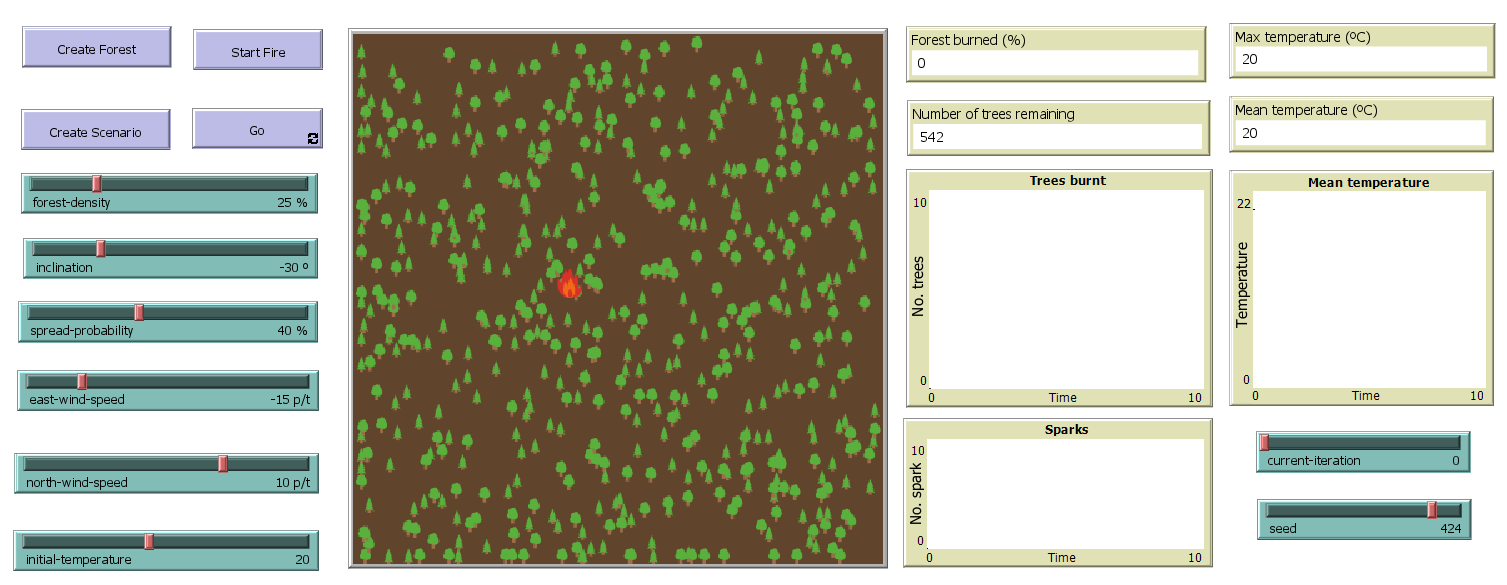
\includegraphics[width=\linewidth]{paper/images/environment}
    \caption{Ambiente de simulação no NetLogo}
    \label{fig:environment}
\end{figure}

Além disso, a fim de poder retratar e avaliar diferentes cenários de incêndio, foi definido um conjunto de variáveis globais, com o recurso aos elementos gráficos do NetLogo, para representar quer propriedades da floresta em si, quer fatores ambientais que podem afetar a propagação do fogo. Entre outros, o modelo prevê os seguintes parâmetros:

\begin{itemize}
    \item \texttt{forest-density} - a densidade da floresta, entre 0 e 100\%;
    \item \texttt{inclination} - a inclinação do terreno, entre \ang{-60} e \ang{60}, responsável pela altitude de cada célula;
    \item \texttt{east-wind-speed} - a velocidade do vento na direção leste (negativa se o vento soprar para o oeste), entre -25 e 25 p/t:
    \item \texttt{north-wind-speed} - a velocidade do vento na direção norte (negativa se o vento soprar para o sul), entre -25 e 25 p/t;
    \item \texttt{initial-temperature} - a temperatura inicial para cada célula do mundo, entre $\SI{0}{\degreeCelsius}$ e $\SI{45}{\degreeCelsius}$;
    \item \texttt{spark-frequency} - a frequência de ocorrência das fagulhas em ticks, por omissão, 150 ticks;
    \item \texttt{spread-probability} - a probabilidade de uma árvore ser incendiada pelo fogo, entre 0 e 100\%;
    \item \texttt{forest-seed} - a semente para o gerador de números aleatórios, entre 0 e 500;
    \item \texttt{current-run} - o número da \textit{run} atual de um dado cenário, entre 0 e 10;
    \item \texttt{iterations} - a lista de entradas contendo um \textit{snapshot} do modelo no final de cada \texttt{tick}.
\end{itemize}

Por fim, os patches também apresentam propriedades únicas, nomeadamente, \texttt{temperature} e \texttt{altitude}, que representam, respetivamente, a temperatura em cada célula à medida que o incêndio se propaga, e a altitude determinada pela inclinação do terreno.

\section{Algoritmo}\label{sec:algorithm}

O objetivo principal deste algoritmo é fornecer uma ferramenta eficiente para modelar e prever o comportamento dos incêndios florestais, permitindo a avaliação dos efeitos de diferentes cenários na propagação do fogo. A simulação baseada em agentes é uma abordagem que considera a interação entre os elementos do ambiente e os agentes que nele atuam, permitindo a modelação de comportamentos complexos e dinâmicos. 

O algoritmo descrito aqui considera fatores como topografia, vento, temperatura, a estrutura da comunidade vegetal e outros elementos relevantes para o comportamento do fogo. A seguir, serão apresentados detalhes do funcionamento do algoritmo e como ele foi implementado para atender aos objetivos.

\SetKwFunction{calcAltitude}{calcAltitude}
\SetKwFunction{random}{random}
\SetKwFunction{plantTree}{plantTree}

\begin{algorithm}
    \caption{Criação da floresta (\texttt{createForest})}\label{alg:create_forest}
    $sparkFrequency \gets 150$\;
    $seed \gets forestSeed$\;
    \For{$patch \in patches$}{
        $altitude \gets \calcAltitude{pxcor}$\;
        $temperature \gets initialTemperature$\;
        \If{\random{$0, 100$} $<$ forestDensity}{
            \plantTree{pxcor, pycor}\;
        }
    }
\end{algorithm}

Em Alg.~\ref{alg:create_forest}, encontra-se detalhado o processo de população da floresta. Este começa por definir a frequência, em ticks, de criação de fagulhas, seguido da atribuição da \textit{seed} responsável pela distribuição de árvores, bem como pela criação do fogo. A cada célula é atribuída uma altitude dependente da sua posição, bem como uma temperatura inicial escolhida pelo utilizador. Também, segundo a densidade da floresta, são plantadas árvores nos diferentes patches.

\SetKwFunction{ignite}{ignite}
\SetKwFunction{saveConfig}{saveConfig}
\SetKwFunction{anyTreesBurning}{anyTreesBurning}
\SetKwFunction{saveIteration}{saveIteration}
\SetKwFunction{saveIterations}{saveIterations}
\SetKwFunction{fire}{fire}

\begin{algorithm}
    \caption{Criação do fogo inicial (\texttt{startFire})}\label{alg:start_fire}
    $patch \gets \random(patches)$\;
    \ignite{patch}\;
    \saveConfig{}\;
    $seed \gets \random{seeds}$\;
    \While{\anyTreesBurning{}}{
        \saveIteration{}\;
        \fire{}\;
    }
    \saveIterations{}\;
\end{algorithm}

Com a floresta plantada, resta criar o fogo inicial, tal como se pode ver em Alg.~\ref{alg:start_fire}. Começa-se por escolher aleatoriamente um patch, no qual é criada a primeira chama. De seguida, são salvas as configurações do cenário em ficheiro YAML, e reiniciada a \textit{seed}. O modelo entra num ciclo condicional, responsável por salvar o estado do modelo em cada iteração e de propagar o incêndio. Após o fim do ciclo, são guardados em ficheiro CSV os resultados das iterações.

\SetKwFunction{spreadFire}{spreadFire}
\SetKwFunction{canSpark}{canSpark}
\SetKwFunction{createSpark}{createSpark}
\SetKwFunction{forward}{forward}
\SetKwFunction{fadeEmbers}{fadeEmbers}
\SetKwFunction{tick}{tick}
\SetKwFunction{create}{create}

\begin{algorithm}
    \caption{Evolução do incêndio (\texttt{fire})}\label{alg:fire}
    \For{$tree \in trees$}{
        \If{isBurning}{
            \If{$color < ``yellow"$}{
                \spreadFire{neighbors, altitude}\;
            }
            \If{$color < ``brown"$}{
                \If{$\random{$0, 1$} < sparkProbability$ {\bf and} $ticksSinceSpark > sparkFrequency$}{
                    \create{spark}\;
                    $ticksSinceSpark \gets 0$\;
                }
                \Else{
                    $ticksSinceSpark \gets ticksSinceSpark + 1$\;
                }
            }
        }
    }
    \For{$spark \in sparks$}{
        \If{$position \neq finalPosition$}{
            \forward{$0.1$}\;
        }
        \Else{
            \ignite{patch-here}\;
        }
    }
    \fadeEmbers{}\;
    \tick{}\;
\end{algorithm}

O Algoritmo~\ref{alg:fire} representa o algoritmo responsável pela evolução do incêndio ao longo da execução do modelo. Em cada tick, as árvores a arder espalham o fogo para as células vizinhas e geram fagulhas, segundo uma certa probabilidade, de acordo com a cor das suas folhas - esta representa o estado da árvore, mais ou menos queimada. Já as fagulhas movem-se em direção à sua posição final, na qual incendeiam as árvores presentes. Por fim, o estado de queima das árvores é atualizado com o procedimento \texttt{fadeEmbers}, responsável por alterar as propriedades da árvore, em particular a sua cor.

\begin{algorithm}
    \caption{Ignição do fogo (\texttt{ignite})}\label{alg:ignite}
    \create{fire}\;
    \For{$tree \in trees{-}here$}{
        \If{{\bf not} ($isBurning$ {\bf and} $isBurnt$)}{
            $isBurning \gets true$\;
        }
    }
\end{algorithm}

Para incendiar as árvores, recorremos ao procedimento \texttt{ignite}, definido em Alg.~\ref{alg:ignite}. Este algoritmo é responsável por criar um agente \textit{fire} na célula atual, bem como de incendiar quaisquer árvores que não estejam a arder na mesma.

\SetKwFunction{towards}{towards}
\SetKwFunction{meanTemperature}{meanTemperature}

\begin{algorithm}
    \caption{Propagação do fogo (\texttt{spreadFire})}\label{alg:spread_fire}
    \KwIn{fireAltitude}
    $probability \gets spreadProbability$\;
    $direction \gets \towards{this}$\;
    \Switch{direction}{
        \Case{\ang{0}}{
            $probability \gets probability - northWindSpeed$\;
        }
        \Case{\ang{90}}{
            $probability \gets probability - eastWindSpeed$\;
        }
        \Case{\ang{180}}{
            $probability \gets probability + northWindSpeed$\;
        }
        \Case{\ang{270}}{
            $probability \gets probability + eastWindSpeed$\;
        }
    }
    $meanTemp \gets \meanTemperature{neighbors}$\;
    $probability \gets probability + \ln^2{(meanTemp + 1)}$\;
    \If{$fireAltitude > altitude$}{
        $probability \gets probability\cdot(1+|\tan(\frac{inclination}{3})|)$\;
    }
    \If{\random{$0, 100$} $<$ probability}{
        \ignite{patch-here}\;
    }
\end{algorithm}

Por fim, temos o algoritmo responsável pela propagação do fogo em si, retratado em Alg.~\ref{alg:spread_fire}. Começa-se por determinar a direção do fogo em relação à célula atual, e por inicializar a probabilidade de propagação com o valor definido pelo utilizador no início do programa. De seguida, consoante a direção do vento, ajusta-se adequadamente esta, tal que o mesmo possa contribuir, positiva ou negativamente para essa propagação. Segue-se o cálculo da temperatura média nas células vizinhas, que é igualmente usada para modificar novamente a propriedade (quanto mais quente estiver o ambiente em redor, melhor se propaga o fogo). Por fim, e porque o fogo tende a subir, quando enfrenta terrenos íngremes, a probabilidade é alterada uma última vez para refletir a inclinação do terreno. Termina-se por incendiar a célula presente, segundo o valor final da probabilidade de propagação.

Todos os detalhes da implementação do modelo de simulação em NetLogo, bem como do módulo desenvolvido em Python para o processamento dos resultados, podem ser consultados no Apêndice~\ref{chapter:appendix}.


    \chapter{Resultados}\label{ch:results}
    Neste capítulo serão apresentados e analisados os resultados da simulação de um incêndio florestal, em quatro cenários distintos. Estes cenários apresentam configurações de modelo semelhantes, diferindo apenas nos seguintes parâmetros: velocidade do vento no sentido Norte e Este, e inclinação do terreno. Todos os valores podem ser consultados na Tab.~\ref{tab:scenarios}.

\begin{table}[tbhp]
    \centering
    \begin{tabular}{c|cccc} 
    \hline
    \textbf{Propriedades} & \textbf{Cenário 1} & \textbf{Cenário 2} & \textbf{Cenário 3} & \textbf{Cenário 4} \\ 
    \hline
    Densidade & 25\% & - & - & - \\
    Carvalhos/pinheiros & 271/272 & - & - & - \\
    Prob. propagação & 0.4 & - & - & - \\
    Temperatura inicial & $\SI{20}{\degreeCelsius}$ & - & - & - \\
    Inclinação & \ang{30} & \ang{-30} & \ang{30} & \ang{-30} \\
    Vento Norte & -10 & -10 & 10 & 10 \\
    Vento Este & 15 & 15 & 15 & 15 \\
    \hline
    \end{tabular}
    \caption{Configurações dos diferentes cenários}
    \label{tab:scenarios}
\end{table}

Cada cenário foi executado onze vezes, e para cada execução foram com guardados em CSV os seguintes parâmetros do modelo: tick, número de árvores ardidas - absoluto, percentual e para cada tipo de árvore, número de fagulhas na floresta, temperatura média e máxima.

\section{Cenário 1}\label{sec:scenario1}

O primeiro cenário apresenta uma inclinação positiva do terreno, de \ang{30}, com vento sudeste de intensidade $(-10, 15)$ \si{\meter\per\second}, ou seja, a favor da propagação do incêndio. O modelo terminou com 71.3\% da floresta ardida, após 3377 ticks, ou 387 árvores em termos absolutos - 205 carvalhos e 182 pinheiros.

De início, o fogo propaga-se rápido, como se pode notar pelas curvas acentuadas das Fig.~\ref{fig:S1ForestBurnt} e \ref{fig:S1TreesBurnt}, acabando por abrandar por volta dos 2000 ticks e estabilizar pouco tempo depois. As fagulhas, dado a sua aleatoriedade e condições específicas de geração, apresentam uma evolução mais errática, evidente pela Fig.~\ref{fig:S1Sparks}, só começando a espalhar-se a partir dos 400 ticks, e atingindo um pico de 15 fagulhas por tick por volta dos 1500 ticks. Dado que a floresta é pouco densa, a temperatura média não ultrapassou os $\SI{330}{\degreeCelsius}$, já a temperatura máxima, atingida após 800 ticks (Fig.~\ref{fig:S1Temp}), foi muito superior, cerca de $\SI{1870}{\degreeCelsius}$.
    
\begin{figure}[H]
    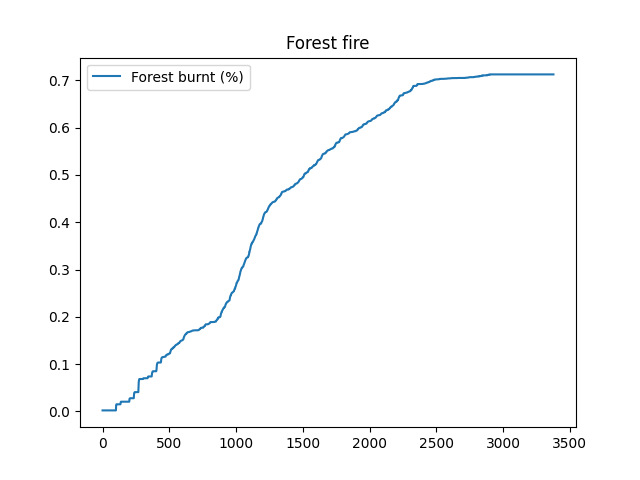
\includegraphics[width=\linewidth]{src/runs/scenario1/forest_fire.png}
    \caption{Cenário 1 - Total de floresta ardida (em percentagem)}
    \label{fig:S1ForestBurnt}        
\end{figure}
    
\begin{figure}[H]
    \centering
    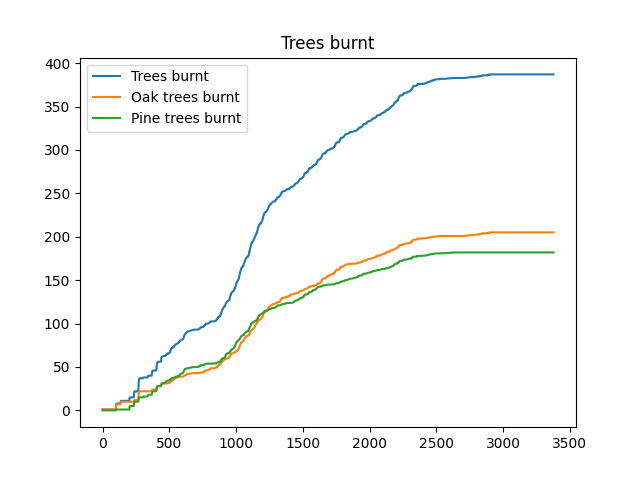
\includegraphics[width=\linewidth]{src/runs/scenario1/trees_burnt.png}
    \caption{Cenário 1 - Total de árvores ardidas}
    \label{fig:S1TreesBurnt}
\end{figure}

\begin{figure}[H]
    \centering
    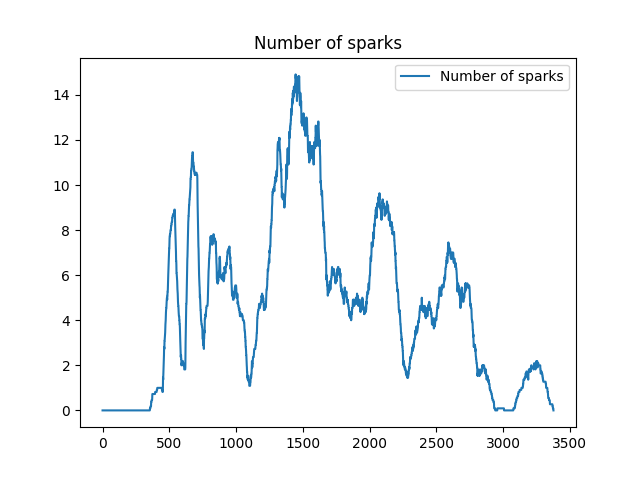
\includegraphics[width=\textwidth]{src/runs/scenario1/sparks.png}
    \caption{Cenário 1 - Evolução do número de fagulhas}
    \label{fig:S1Sparks}
\end{figure}

\begin{figure}[H]
    \centering
    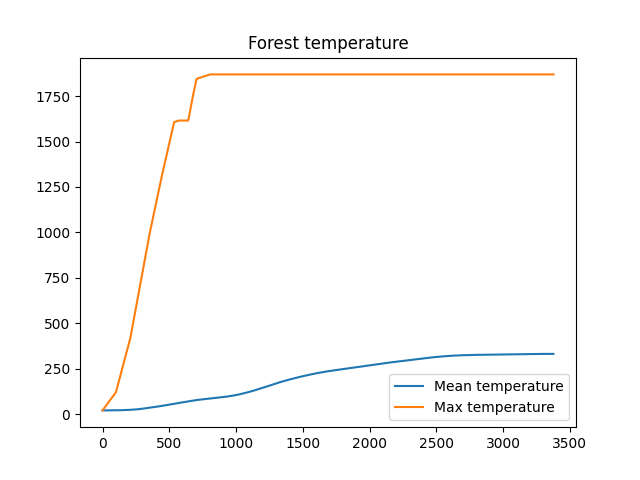
\includegraphics[width=\textwidth]{src/runs/scenario1/temperature.png}
    \caption{Cenário 1 - Evolução da temperatura média e máxima}
    \label{fig:S1Temp}
\end{figure}

\section{Cenário 2}\label{sec:scenario2}

O segundo cenário apresenta uma inclinação negativa do terreno, de \ang{-30}, com vento sudeste de intensidade $(-10, 15)$ \si{\meter\per\second}, ou seja, contra a propagação do incêndio. O modelo terminou com 71.4\% da floresta ardida, após 3359 ticks, ou 388 árvores em termos absolutos - 206 carvalhos e 182 pinheiros.

Apesar das condições adversas, o fogo propagou-se rapidamente, à semelhança do que aconteceu em \ref{sec:scenario1}. Quando analisadas as curvas das Fig.~\ref{fig:S2ForestBurnt} e \ref{fig:S2TreesBurnt}, torna-se evidente que o modelo teve uma evolução quase idêntica, porventura graças à alta probabilidade de propagação (40\%). Novamente, as fagulhas, apresentam uma evolução mais instável, evidente pela Fig.~\ref{fig:S2Sparks}, atingindo um pico de 16 fagulhas por tick por volta dos 1400 ticks. Por fim, a temperatura média ficou-se igualmente pelos $\SI{330}{\degreeCelsius}$, já a temperatura máxima, atingida após 800 ticks (Fig.~\ref{fig:S1Temp}), foi à volta de $\SI{1870}{\degreeCelsius}$.

\begin{figure}[H]
    \centering
    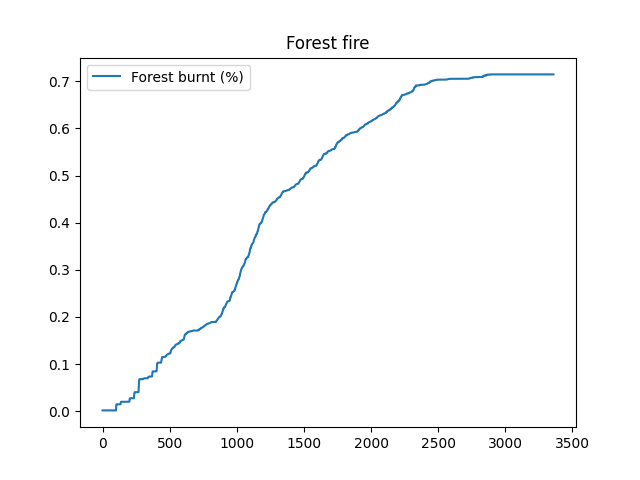
\includegraphics[width=\textwidth]{src/runs/scenario2/forest_fire.png}
    \caption{Cenário 2 - Total de floresta ardida (em percentagem)}
    \label{fig:S2ForestBurnt}
\end{figure}

\begin{figure}[H]
    \centering
    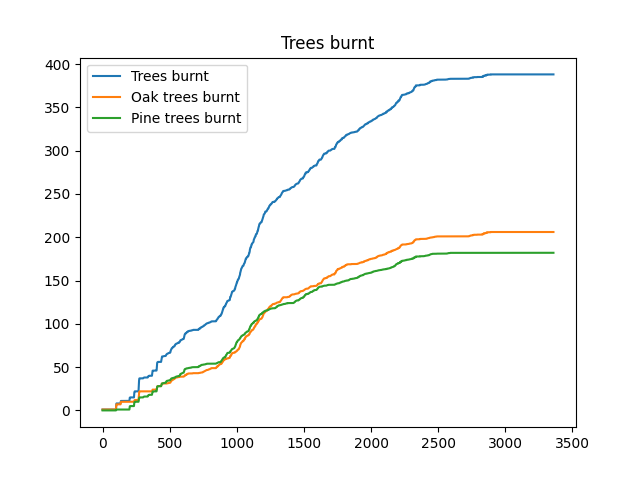
\includegraphics[width=\textwidth]{src/runs/scenario2/trees_burnt.png}
    \caption{Cenário 2 - Total de árvores ardidas}
    \label{fig:S2TreesBurnt}
\end{figure}

\begin{figure}[H]
    \centering
    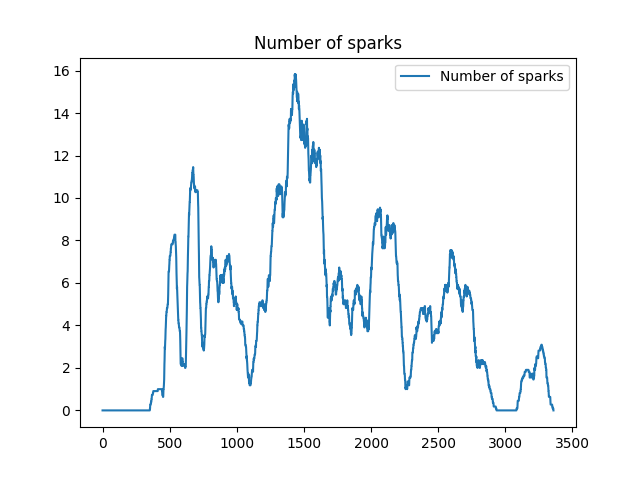
\includegraphics[width=\textwidth]{src/runs/scenario2/sparks.png}
    \caption{Cenário 2 - Evolução do número de fagulhas}
    \label{fig:S2Sparks}
\end{figure}

\begin{figure}[H]
    \centering
    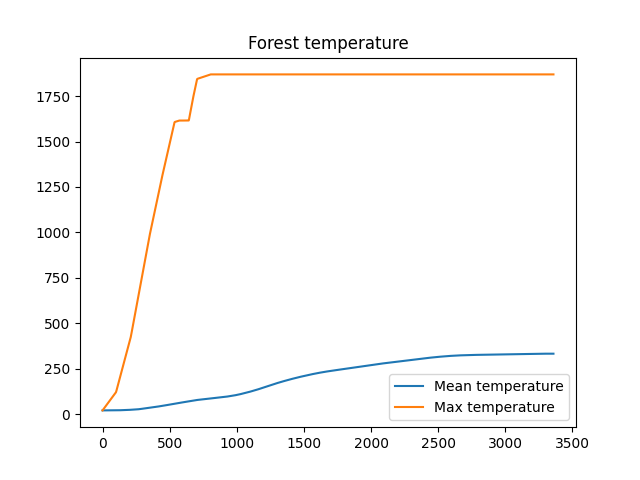
\includegraphics[width=\textwidth]{src/runs/scenario2/temperature.png}
    \caption{Cenário 2 - Evolução da temperatura média e máxima}
    \label{fig:S2Temp}
\end{figure}

\section{Cenário 3}\label{sec:scenario3}

O terceiro cenário apresenta uma inclinação positiva do terreno, de \ang{30}, com vento noroeste de intensidade $(10, -15)$ \si{\meter\per\second}, ou seja, contra da propagação do incêndio. O modelo terminou com 93.4\% da floresta ardida, após 3042 ticks, ou 508 árvores em termos absolutos - 250 carvalhos e 258 pinheiros. 

O incêndio foi capaz de destruir uma maior área da floresta, visível em Fig.~\ref{fig:S3ForestBurnt}, em menos tempo que os cenários anteriores. Ao nível do tipo de árvores ardidas, dada a sua idêntica distribuição pelo terreno, não houve variações significativas entre pinheiros e carvalhos, como se pode constatar pela Fig.~\ref{fig:S3TreesBurnt}. Também ao nível das fagulhas criadas, é possível notar um aumento considerável, com o modelo a atingir um pico de 18.5 fagulhas por tick por volta 
1500 ticks (Fig.~\ref{fig:S3Sparks}). A temperatura média final foi ligeiramente superior, na ordem dos $\SI{412}{\degreeCelsius}$, já a temperatura máxima, atingida após 800 ticks (Fig.~\ref{fig:S3Temp}), manteve-se nos $\SI{1870}{\degreeCelsius}$.

\begin{figure}[H]
    \centering
    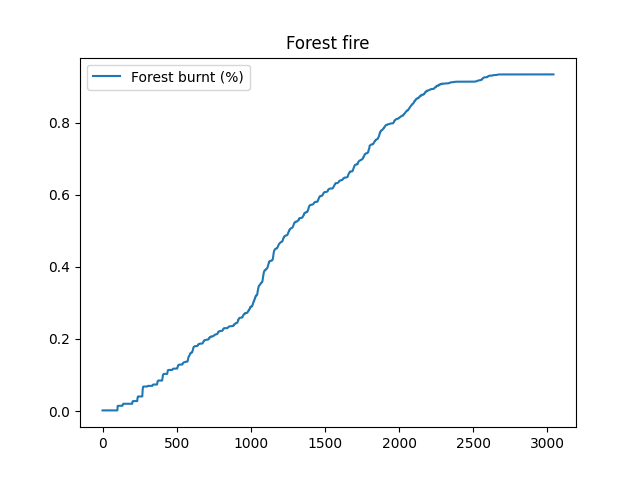
\includegraphics[width=\textwidth]{src/runs/scenario3/forest_fire.png}
    \caption{Cenário 3 - Total de floresta ardida (em percentagem)}
    \label{fig:S3ForestBurnt}
\end{figure}

\begin{figure}[H]
    \centering
    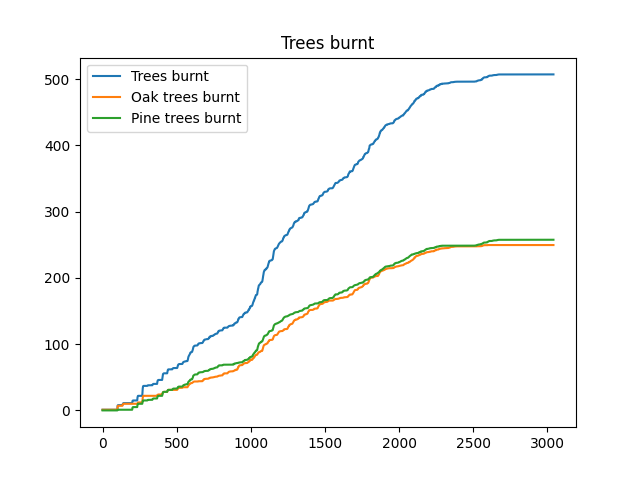
\includegraphics[width=\textwidth]{src/runs/scenario3/trees_burnt.png}
    \caption{Cenário 3 - Total de árvores ardidas}
    \label{fig:S3TreesBurnt}
\end{figure}

\begin{figure}[H]
    \centering
    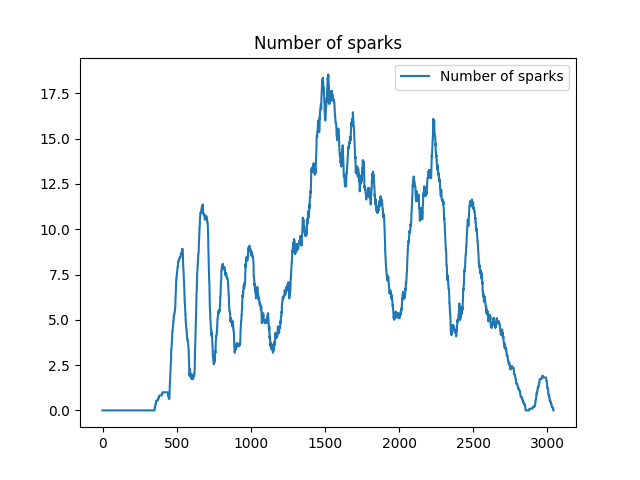
\includegraphics[width=\textwidth]{src/runs/scenario3/sparks.png}
    \caption{Cenário 3 - Evolução do número de fagulhas}
    \label{fig:S3Sparks}
\end{figure}

\begin{figure}[H]
    \centering
    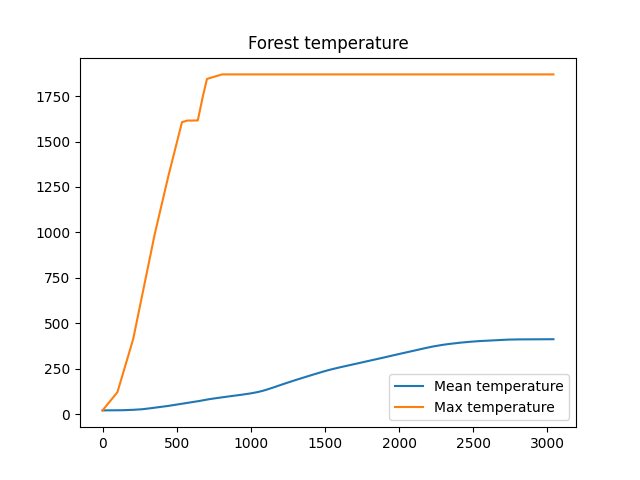
\includegraphics[width=\textwidth]{src/runs/scenario3/temperature.png}
    \caption{Cenário 3 - Evolução da temperatura média e máxima}
    \label{fig:S3Temp}
\end{figure}

\section{Cenário 4}\label{sec:scenario4}

O quarto e último cenário apresenta uma inclinação negativa do terreno, de \ang{-30}, com vento noroeste de intensidade $(10, -15)$ \si{\meter\per\second}, ou seja, a favor da propagação do incêndio. O modelo terminou com 93.3\% da floresta ardida, após 3103 ticks, ou 507 árvores em termos absolutos - 250 carvalhos e 257 pinheiros.

Este cenário apresenta condições de vento idênticas ao descrito em \ref{sec:scenario3}, pelo que o modelo em si também evidenciou uma evolução do incêndio similar, quer ao nível da floresta ardida (Fig.~\ref{fig:S4ForestBurnt}), quer ao nível do tipo de árvores ardidas (Fig.~\ref{fig:S4TreesBurnt}). No que concerne as fagulhas, o modelo atingiu um pico marginalmente superior, de 18.5 fagulhas por tick por volta 
1500 ticks (Fig.~\ref{fig:S4Sparks}). A temperatura média final foi por volta de $\SI{411}{\degreeCelsius}$, já a temperatura máxima, atingida após 800 ticks (Fig.~\ref{fig:S3Temp}), manteve-se nos $\SI{1870}{\degreeCelsius}$.

\begin{figure}[H]
    \centering
    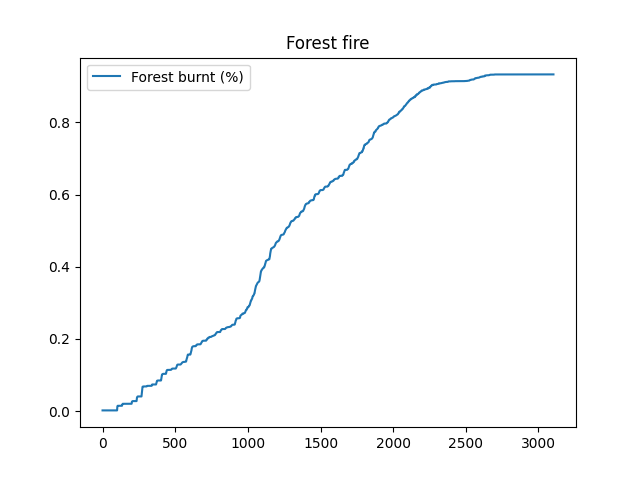
\includegraphics[width=\textwidth]{src/runs/scenario4/forest_fire.png}
    \caption{Cenário 4 - Total de floresta ardida (em percentagem)}
    \label{fig:S4ForestBurnt}
\end{figure}

\begin{figure}[H]
    \centering
    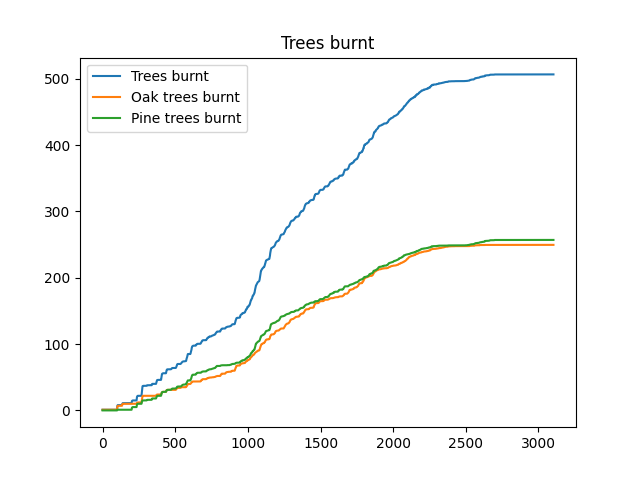
\includegraphics[width=\textwidth]{src/runs/scenario4/trees_burnt.png}
    \caption{Cenário 4 - Total de árvores ardidas}
    \label{fig:S4TreesBurnt}
\end{figure}

\begin{figure}[H]
    \centering
    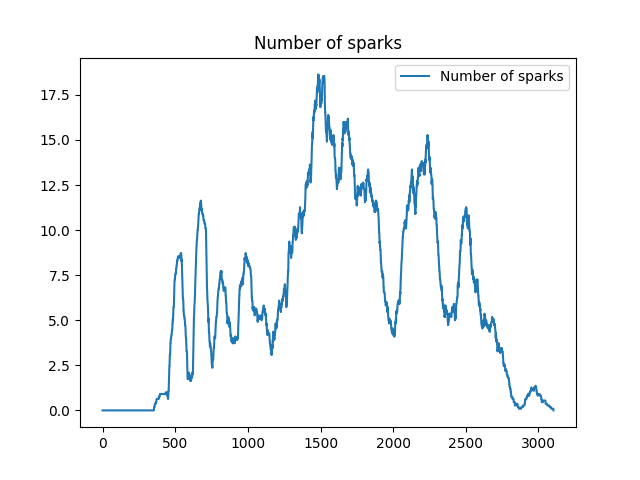
\includegraphics[width=\textwidth]{src/runs/scenario4/sparks.png}
    \caption{Cenário 4 - Evolução do número de fagulhas}
    \label{fig:S4Sparks}
\end{figure}

\begin{figure}[H]
    \centering
    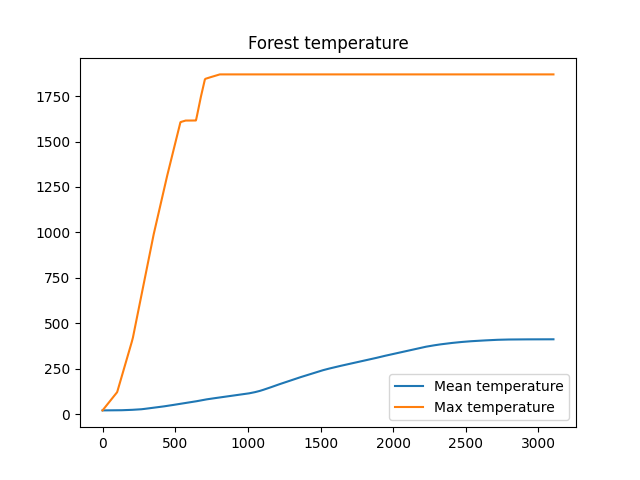
\includegraphics[width=\textwidth]{src/runs/scenario4/temperature.png}
    \caption{Cenário 4 - Evolução da temperatura média e máxima}
    \label{fig:S4Temp}
\end{figure}


    \chapter{Conclusões}\label{ch:conclusoes}
    Neste trabalho, desenvolveu-se um sistema computacional com agentes racionais utilizando a ferramenta NetLogo, com o objetivo de simular a propagação de um incêndio florestal considerando diferentes fatores ambientais. Foram analisados quatro cenários distintos, variando a inclinação do terreno e a direção do vento.

Os resultados obtidos não foram conforme o esperado, uma vez que os cenários com vento a favor e contra a inclinação apresentaram valores contraditórios. As nossas expectativas eram de que a propagação do incêndio seria maior nos casos em que o vento estivesse a favor da inclinação, e menor nos casos em que o vento estivesse contra a inclinação. No entanto, o que se observou foi que a percentagem da floresta ardida e outros parâmetros analisados não seguiram essa lógica.

Uma possível explicação para os resultados contraditórios pode ser a simplificação de alguns elementos do modelo, bem como a aleatoriedade de fatores como a geração de fagulhas. Outro fator que poderá ter contribuído para essa contradição é a alta probabilidade de propagação utilizada, que pode ter mascarado o efeito esperado da direção do vento e da inclinação do terreno.

A partir das conclusões deste trabalho, é possível sugerir melhorias no modelo de simulação para investigação futura. Estas melhorias podem incluir a consideração de outros fatores ambientais, como a humidade do ar e do solo, e uma análise mais aprofundada das probabilidades de propagação. Além disso, a realização de mais testes com diferentes configurações de parâmetros pode ajudar a compreender melhor as discrepâncias observadas.

Concluímos que a simulação baseada em agentes é uma ferramenta valiosa no estudo de incêndios florestais, permitindo aos investigadores compreender melhor as complexas interações e comportamentos envolvidos. Essas simulações têm sido usadas para explorar tópicos como estratégias de combate a incêndios, impacto do clima e topografia, e fatores humanos na gestão de incêndios. A melhor compreensão destes fatores pode levar a decisões mais informadas e práticas mais eficazes, tornando a simulação baseada em agentes uma ferramenta essencial na redução do impacto dos incêndios florestais. Embora os resultados não tenham sido os esperados, o trabalho realizado neste projeto servirá como base para futuras investigações e melhorias no campo da prevenção e combate a incêndios florestais.

    \appendix


    \chapter{Anexos dos ficheiros fonte}\label{ch:appendix}


    \section{Especificação do modelo de simulação em NetLogo}\label{sec:model_spec}
    \inputminted[breaklines]{nl-lexer.py:NetLogoLexer -x}{../src/forest_fire.nlogo}


    \section{Especificação do módulo de processamento de dados em Python}\label{sec:data_proc}

    \subsection{Programa principal}\label{subsec:programa-principal}
    \inputminted[breaklines]{python}{../src/main.py}

    \subsection{Definição da classe Scenario}\label{subsec:definicao-da-classe-scenario}
    \inputminted[breaklines]{python}{../src/forestfire/scenario.py}

    \subsection{Definição da classe Run}\label{subsec:definicao-da-classe-run}
    \inputminted[breaklines]{python}{../src/forestfire/run.py}

    \bibliographystyle{IEEEtran}
    \bibliography{references}

\end{document}

